\chapter{Основы Linux}

\begin{frame}{Основы ОС Linux}

	\begin{block}{Вопрос}
	Почему Linux является самой популярной
	свободной операционной системой?
	\end{block}

	\pause

	\begin{block}{Ответ}
	\begin{itemize}
		\item \textcopyleft -- Copyleft
		\item ``Философия'' Unix
		\item Открытые стандарты
	\end{itemize}
	\end{block}

\end{frame}


\chapter[Принципы]{Базовые принципы ОС Linux}

\subsection{GNU/Linux}

\mode<all>{\input{../../slides/intro/vocabulary}}

\subsection{Лицензии}

\mode<all>{\begin{frame}{Авторское право и лицензии}

	\begin{block}{Авторское право}
		 Возникает по факту создания ПО 

		\begin{itemize}
			\item Неимущественные права
			\item Имущественные права
		\end{itemize}
	\end{block}

	\pause

	\begin{block}{Лицензии}
		Лицензия -- средство передать какие-либо права на продукт либо его часть.

		Необходима для защиты авторских прав. 
		Средство для возможности законно пресечь несанкционирование копирование,  использование или распространение ПО. 
	\end{block}
\end{frame}


\begin{frame}{Лицензии: открытые и свободные}
	\begin{block}{ Р.Столлман: 4 свободы}
		\begin{itemize}
			\item Свобода 0: Свобода запускать программу в любых целях.
			\item Свобода 1: Свобода изучения работы программы и адаптация её к вашим нуждам. 
				Доступ к исходным текстам является необходимым условием.
			\item Свобода 2: Свобода распространять копии,  так что вы можете помочь вашему товарищу.
			\item Свобода 3: Свобода улучшать программу и публиковать ваши улучшения,
				так что всё общество выиграет от этого.
				Доступ к исходным текстам является необходимым условием.
		\end{itemize}
	\end{block}
\end{frame}


\begin{frame}{Лицензии: permissive}
	\begin{columns}
	\column{0.3\textwidth}
		\center\includegraphics[width=2cm,natwidth=144,natheight=144]{../../slides/intro/three-arrows@2x.png}

	\column{0.6\textwidth}

	\begin{itemize}
		\item BSD
		\item MIT
		\item Apache
	\end{itemize}
	\end{columns}

	\begin{block}{I want it simple and permissive.}
		\begin{itemize}
			\item практически не ограничивают свободу действий пользователей ПО и разработчиков, работающих с исходным кодом.
			\item По своему духу, распространение работы под пермиссивной лицензией схоже с помещением работы в общественное
				достояние, но не требует отказа от авторского права.
		\end{itemize}
	\end{block}

\end{frame}


\begin{frame}{\textcopyleft -- Copyleft}

	\begin{columns}
	\column{0.3\textwidth}
		\center\includegraphics[width=2cm,natwidth=144,natheight=138]{../../slides/intro/circular@2x.png}

	\column{0.6\textwidth}

	\begin{itemize}
		\item GPL
		\item LGPL
		\item AGPL
	\end{itemize}
	\end{columns}


	\begin{block}{I care about sharing improvements.}
	
	Авторское лево -- концепция и практика использования законов авторского права для обеспечения 
	невозможности ограничить любому человеку право использовать,  изменять и распространять как 
	исходное произведение,  так и произведения,  производные от него.
	\end{block}


	При копилефте все производные произведения должны распространяться под той же лицензией,
	что и оригинальное произведение.

\end{frame}



}

\subsection{Принципы проектирования переносимых программ}

\mode<all>{\input{../../slides/intro/unixway}}

\section{Дистрибутивы ОС Linux}

\mode<all>{\begin{frame}{Дистрибутив ОС GNU/Linux}
	\begin{block}{ Определение}
		\only<1>{\center{\bf{?}}}
		\pause
		\only<2->{Набор программного обеспечения на базе ядра Linux, распространяющийся как единое целое.}
	\end{block}
\end{frame}


\begin{frame}{Задачи дистрибутива}
	\begin{itemize}
		\item Предоставление комплекта ПО (ядро + утилиты)
		\item Средства установки и настройки
		\item Средства обновления
	\end{itemize}
\end{frame}

\begin{frame}{Различия между дистрибутивами}

	\only<1>{\Large\center{\bf{?}}}
	\pause
	\only<2->{\Large\center{\bf{Цели!!!}}}

	\bigskip
	\normalsize

	\pause

	\begin{itemize}
		\begin{columns}
		\column{0.4\textwidth}
			\item Инсталлятор
			\item Первичные настройки
			\item Средства управления
			\item Набор ПО
		\column{0.4\textwidth}
			\item Менеджер пакетов
			\item Формат распространения ПО
			\item Пути к файлам
			\item Система сборки ПО
		\end{columns}
	\end{itemize}
\end{frame}

\begin{frame}{Дистрибутивы}
	\begin{itemize}
		\begin{columns}
		\column{0.3\textwidth}
			\item RedHat
			\item Fedora Core
			\item CentOS
			\item Scientific Linux
			\item Oracle Unbreakable Linux
		\column{0.3\textwidth}
			\item Slackware 
			\item Gentoo
			\item Arch
			\item OpenSUSE
			\item ALT Linux 
		\column{0.3\textwidth}
			\item Debian
			\item Ubuntu
			\item Mint
			\item Knoppix
			\item BackTrack
		\end{columns}
	\end{itemize}
\end{frame}
}

\section{Процесс загрузки ОС Linux}

\subsection{Этапы загрузки}

\mode<all>{\begin{frame}{Процесс загрузки GNU/Linux}
	\scriptsize
	\begin{enumerate}
		\item BIOS
		\item Master Boot Record (MBR)
			\pause
		\item Загрузка загрузчика 
		\begin{itemize}
		\footnotesize
			\item Stage 1 -- Первичный загрузчик
			\item Stage 1,5 -- Загрузка ядра загрузчика и драйвера ФС
			\item Stage 2 -- загрузчик читает конфигурацию, загружает ядра и образ initrd (initial-RAM disk) в память
                        \item Передает управление ядру
		\end{itemize}

		\item Запуск программы инициализации в initrd, загрузка драйверов файловых систем (LVM, RAID, NFS)
			\pause
		\item Нахождение и монтирование корневого раздела
			\pause
		\item Запуск программы init
		\begin{itemize}
		\footnotesize
			\item Монтирование оставшихся разделов ФС
			\item Запуск демонов для заданного уровня загрузки (runlevel)
			\item Выдает приглашение пользователю. 
		\end{itemize}

	\end{enumerate}
\end{frame}
}

\subsection{Ядро Linux}

\mode<all>{\begin{frame}{Задачи ядра Linux}
	\begin{itemize}
		\item Инициализация системы
		\item Управление процессами и потоками
		\item Управление памятью
		\item Управление файлами
		\item IPC (Inter Process Communication)
		\item Разграничение доступа
		\item Сетевые возможности
		\item Интерфейс доступа к возможностям ядра
	\end{itemize}
	%Выполнить команду dmesg и найти строки инициализации памяти, CPU, дисковой подсистемы, CPU.
\end{frame}


\begin{frame}{Ядро}

	Ядро ОС Linux является модульным. 

	\begin{block}{Модули}
		\begin{itemize}
			\item В виде отдельных файлов
			\item "Вкомпилированные" в ядро
		\end{itemize}
	\end{block}

	\bigskip
	%Список загруженных модулей: {\tt cat /proc/modules } либо {\tt lsmod}
\end{frame}


\begin{frame}{Параметры ядра}
	
	Полный список: {\tt Documentation/kernel-parameters.txt}

	\begin{block}{Некоторые часто применяемые параметры}
		\begin{itemize}
			\begin{columns}
			\column{0.3\textwidth}
				\item console=ttyS0,9600
				\item debug
				\item init=/sbin/init
				\item loglevel=[0-7]
				\item maxcpus=[num]
			\column{0.3\textwidth}
				\item mem=nn[KMG]
				\item noacpi
				\item noapic
				\item panic=nn (sec)
				\item resume=/dev/sda2
			\column{0.3\textwidth}
				\item ro
				\item rw
				\item root=/dev/sda1
				\item rootdelay=nn (sec)
				\item rootwait
				\item vga=<num>|ask
			\end{columns}
		\end{itemize}
	\end{block}

	Параметры переданные ядру во время загрузки: {\tt /proc/cmdline} \\

        Программы могут использовать /cmdline, например установщик ОС Anaconda \\

	Модулям можно передавать параметры используя синтаксис: {\tt module.param=value} \\
\end{frame}
}

\subsection{Userspace}

\mode<all>{\input{../../slides/intro/initrd}}

\mode<all>{\begin{frame}{init}
	Менеджер управления работой системой и сервисами.
	
	\bigskip

	\center{\large PID = 1}

	\bigskip

	\begin{block}{Наиболее известные}
		\begin{itemize}
			\item SysVInit
			\item systemd
			\item upstart
		\end{itemize}
	\end{block}
\end{frame}

\begin{frame}{SysVInit}
	\begin{block}{Управление}
		\begin{itemize}
			\item kernel boot parameters: <N> -- runlevel
			\item утилита {\tt runlevel}
			\item утилита {\tt init}
		\end{itemize}
	\end{block}

	\scriptsize
	\begin{block}{Runlevel}
		\begin{table}
			\begin{tabular}{| c | l | }
			\hline
			Runlevel & Описание\\
			\hline
			0	& Выключить систему \\
			1,s,single & Однопользовательский режим \\
			2	& Многопользовательский режим без графики. Без сетевых сервисов.\\
			3	& Многопользовательский режим без графики. Полноценная сеть. \\
			4	& Определяется на хосте\\
			5	& Многопользовательский режим с графикой.\\
			6	& Перезагрузка\\
			emergency & Аварийная оболочка \\
			\hline
			\end{tabular}
		\end{table}
	\end{block}
\end{frame}

\begin{frame}{SysVInit: сервисы}
	\begin{block}{Управление}
		\begin{itemize}
			\item утилита {\tt service}
			\item утилита {\tt chkconfig}
		\end{itemize}
	\end{block}

	\begin{block}{Сервисы}
		\begin{itemize}
			\item {\tt /etc/rc.d/init.d}
			\item {\tt /etc/rc.d/rc.N}\footnote{N=runlevel}
		\end{itemize}
	\end{block}
\end{frame}

\begin{frame}{systemd}
	\begin{block}{Управление}
		\begin{itemize}
			\item kernel boot parameters\\
				{\tt systemd.unit=rescue.target} \\
			\item утилита {\tt systemctl} \\
				{\tt systemctl isolate multi-user.target} \\
				{\tt systemctl set-default single.target}
		\end{itemize}
	\end{block}

	\begin{block}{targets}
		\tiny
		\begin{table}
			\begin{tabular}{| c | l | l | }
			\hline
			Runlevel & Описание\\
			\hline
			0	& poweroff.target & Выключить систему \\
			1,s,single & rescue.target  & Однопользовательский режим \\
			2	& multi-user.target & Многопользовательский режим без графики. Без сетевых сервисов.\\
			3	& multi-user.target & Многопользовательский режим без графики. Полноценная сеть. \\
			4	& multi-user.target & Определяется на хосте\\
			5	& graphical.target & Многопользовательский режим с графикой.\\
			6	& reboot.target & Перезагрузка\\
			emergency & emergency.target & Аварийная оболочка \\
			\hline
			\end{tabular}
		\end{table}
	\end{block}
\end{frame}

\begin{frame}{systemd: сервисы}
	\begin{block}{Управление}
		\begin{itemize}
			\item утилита {\tt systemctl}
		\end{itemize}
	\end{block}

	\begin{block}{Сервисы}
		\begin{itemize}
			\item {\tt /lib/systemd/system/}
			\item {\tt /etc/systemd/system/}
		\end{itemize}
	\end{block}
\end{frame}
}

\subsection{Практика}

\mode<all>{\begin{frame}{Практическое задание}
	\begin{enumerate}
		\item Загрузить ОС по умолчанию
		\item Посмотреть используемые параметры ядра 
		\item Посмотреть список загруженных модулей
			\pause
		\item Переопределить init на sh
		\item SysRq. {\bf R}eboot {\bf E}ven {\bf I}f {\bf S}ystem {\bf U}tterly {\bf B}roken
			\pause
		\item Загрузить ядро с "урезанным" количеством памяти
		\item Отключить 1 или несколько процессоров
			\pause
		\item Посмотреть текущий runlevel
		\item Посмотреть список сервисов
	\end{enumerate}
\end{frame}
}


\chapter{Командная строка}

\section{Интерфейс командной строки}
\mode<all>{% Тема. Командная строка. 
% Показать примеры использования. Рассказать о преимуществах и недостатках в
% сравненни с графическим "оконным" интерфейсом. 
% Ознакомить с назначениме  эмулятора терминала и об реализациях.

\begin{frame}{Примеры использования командной строки}
        CLI (Command Line Interface)
	\begin{columns}
	\column{0.5\textwidth}
        \begin{itemize}
            \item интерфейс настройки сетевого оборудования
            \item чаты
            \item компьютерные игры
            \item операционные системы
        \end{itemize}
	\column{0.5\textwidth}
	% insert picture of Quake 
    \includegraphics[height=0.4\textheight]{../../slides/cmdline/330px-Tremulous_console.png}
	\end{columns}
\end{frame}

\begin{frame}{Преимущества командной строки}
	\begin{itemize}
                \item Используют мало ресурсов
		\item Работа через сеть либо RS232, в том числе медленную
		\item Быстрый доступ к командам системы
		\item Отладка сообществом CLI приложения проще
		\item Легкость автоматизации
	\end{itemize}
\end{frame}

\begin{frame}{Недостатки командной строки}
	\begin{itemize}
		\item Oтсутствуют возможности обнаружения (discoverabililty)
		\item Отсутствие «аналогового» ввода.
		\item Необходимость изучения синтаксиса команд и запоминания сокращений.  (синтаксис может различаться)
		\item Без автодополнения, ввод длинных и содержащих спецсимволы параметров с клавиатуры может быть затруднительным
	\end{itemize}
\end{frame}

\note { 
Примеры приложений которые лучше выглядят в графическом режиме браузер,
редакторы видео и графики. Поэтому пользователь при работе, как правило,
совмещает оба интерфейса: использует графическое окружениe в сочетании с
интерфейсом командной строки. 
В графическом окружении интерфейса командной строки предоставляют приложения -
эмуляторы терминала. 
реализации - для графической системы X Window xterm, rxvt. Для GNOME
gnome-terminal, для KDE konsole, Yakuake (Yet Another Kuake выезжает по нажатии
тильды ~ как Quake)  
Дополнительные замечания:
Терминал - устройство для ввода вывода информации, уже устарел.
Графические приложения можно запускать из командной строки. 
}
}

\section{Командная оболочка (shell)}

\mode<all>{\input{../../slides/cmdline/shell-intro}}

\section{Don't panic! Получение помощи}

\mode<all>{\begin{frame}[fragile]{From FAQ How To Ask Questions The Smart Way}
Before You Ask try to find an answer
  \begin{itemize}
	  \item by reading (RTFM): manual, FAQ, archives of the forum, by searching the Web;
	  \item by inspection or experimentation;
	  \item by asking a skilled friend;
	  \item by reading the source code;
    \end{itemize}
\end{frame}


\begin{frame}[fragile]{Встроенная документация}
\begin{itemize}
    \item \textbf{man} - помощь по внешним командам
    \pause
    \item \textbf{info} - расширенная помощь по некоторым командам (texinfo format)
    \pause
    \item \textbf{find /usr/share/doc/} - файлы документации поставляемые вместе с приложением
    \item \textbf{-h, --help option} - встроенная в приложение справка
    \item \textbf{help} - встроенная помощь по внутренним командам bash (также man bash)
\end{itemize}
\end{frame}

\begin{frame}[fragile]{Основное о man}
      \textbf{man \textless command\_name\textgreater }

	\begin{block}{Example: show uptime manual page}
		{\tt man uptime}
	\end{block}

		\begin{itemize}
			\item Прочитайте {\tt man man} !
		\end{itemize}

\end{frame}

\begin{frame}[fragile]{man page navigation}
		\begin{itemize}
			\item \textbf{up, down} - scroll one line
			\item \textbf{q} - exit
			\item \textbf{/pattern} - search pattern
			\item \textbf{n} - next text pattern
			\item \textbf{N} - repeat search in back direction
			\item \textbf{h} - help
		\end{itemize}
\end{frame}

\begin{frame}[fragile]{Page structure}
		\begin{itemize}
			\item NAME
			\item SYNOPSIS
			\item DESCRIPTION
			\item EXAMPLES
			\item SEE ALSO
		\end{itemize}
\end{frame}

\begin{frame}[fragile]{Разделы помощи}
	\begin{itemize}
		\item[1] Основная секция(юзерские программы)
		\item[2] Syscalls
		\item[3] С library
		\item[5] Конфигурационные файлы
		\item[8] Системные службы
	\end{itemize}
\end{frame}

\begin{frame}[fragile]{More than one section of the manual}
	name(section)  \\ 
	\textbf{man(1)} and \textbf{man(7)}, or \textbf{exit(2)} and \textbf{exit(3)} \\
     \begin{block}{Example: show manual in section 5 and 1}
        \begin{lstlisting}
man -f passwd #or whatis passwd 
man 5 passwd; man 1 passwd; man -wa passwd
        \end{lstlisting}
    \end{block}
\end{frame}

\begin{frame}[fragile]{Поиск по страницам помощи}
     \begin{block}{Упражнение. Поиск страниц с ключевым словом.}
        \begin{lstlisting}
man -f passwd #or whatis passwd 
man -k passwd #or apropos passwd 
whatis  -l -w '*'
man -s 3 -Kw passwd
        \end{lstlisting}
    \end{block}
\end{frame}


%\begin{frame}[fragile]{Чему научились}
%  \begin{itemize}
%  \item Как спрашивать у сообщества
%  \item Умеем использовать 3 источника получения информации man, info, help
%  \item Как перемещаться по страницам помощи info и man
%  \item Иcкать в системе помощи man и запрашивать из одного из 8-ми разделов 
%  \end{itemize}
%\end{frame}
}

\section{Навигация по файловой системе}

\mode<all>{\begin{frame}[fragile]{Путь к файлу.}
      \begin{itemize}
        \item Имя файла
                \begin{itemize}
                    \item чувствительно к регистру
                    \item / разделяет директории
                    \item - \textbackslash <Space> специальные символы 
                    \item . скрытый файл
                \end{itemize}
        \item \alert{Полное имя файла} (absolute pathname) начинается с /
        \item \alert{Относительное имя файла} (relative pathname) начинается с
        любого другого символа. Поиск файла производится относительно
        \alert{текущей директории} (current working directory).
      \end{itemize}

      \begin{block}{Примеры}
        ./ - текущая директория

        ../ - предыдущая директория

        ../../usr/bin/ls

        /usr/bin/ls
      \end{block}
\end{frame}

\begin{frame}[fragile]{Навигация по файловой системе}
      \begin{itemize}
		  \item {\tt pwd} -- имя текущей директории (help pwd)
		  \item {\tt ls} -- список файлов в директории. По умолчанию в текущей (man ls)
		  \item {\tt cd} -- смена текущей директории (help cd)
      \end{itemize}
      \begin{block}{Упражнение. Заходим в /usr/bin/ и просматриваем список доступных команд.}
	\begin{lstlisting}
	pwd
	cd /usr/bin/
	pwd
	ls
	cd -	
	pwd
	\end{lstlisting}
      \end{block}
\end{frame}

\begin{frame}[fragile]{Просмотр типов файлов}
      \begin{block}{Упражнение. Символьное обозначение типа файла.}
Первая буква вывода команды ls -l обозначает тип файла. 
Tip. Команды file позволяет определить тип файла. Ключ -d для работы с
директорией. 

/dev/zero

/dev/sda 

.. 

/bin/sh 

/dev/log

/dev/stdout
      \end{block}
\end{frame}

\begin{frame}[fragile]{Команды для работы с файлами}
	\begin{itemize}
		\begin{columns}
		\column{0.2\textwidth}
			\item touch
			\item ln
			\item mkdir
			\item mknod
			\item mkfifo

		\column{0.2\textwidth}
			\item cp
			\item mv
			\item rm
			\item rmdir
			\item file
			\item install

		\column{0.4\textwidth}
			\begin{block}{Упражнение}
				\begin{enumerate}
					\item Создать иерархию директорий
						\begin{lstlisting}
dir1/dir1.1/dir1.1.1
dir1/dir1.2/dir1.2.1
dir1/dir1.2/dir1.2.2
						\end{lstlisting}
					\item Внутри каждой создать файл
					\item Удалить все созданное
				\end{enumerate}
			\end{block}
			
		\end{columns}
	\end{itemize}
\end{frame}
}

\mode<all>{
\begin{frame}{Детали реализации}
  \begin{itemize}
    \item \alert{VFS - virtual file system} - файлы и каталоги отображаются в единое дерево, независимо от их физического расположения.
  \end{itemize}
  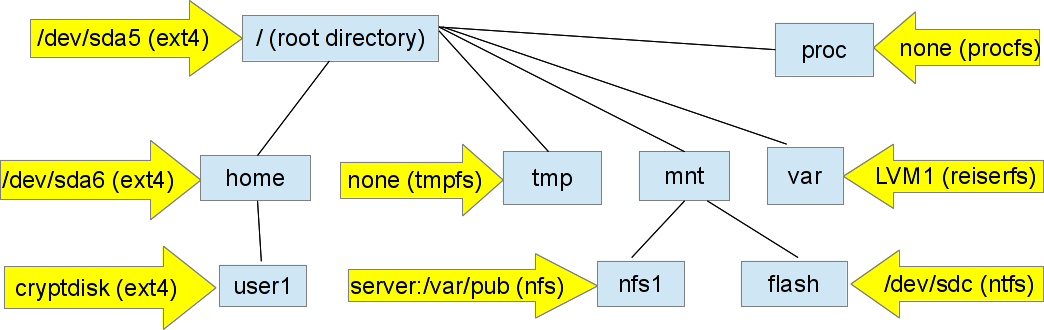
\includegraphics[height=3.5cm]{vfs-and-devices}
\end{frame}

\begin{frame}{Монтирование}
  \begin{itemize}
    \item \alert{Монтирование} - процесс отображения содержимого устройства в указанную папку файловой системы.
    \item Команды:
      \begin{itemize}
        \item монтировать - ( \alert{mount} ) 
        \item размонтировать ( \alert{umount} )
      \end{itemize}
    \item \alert{mount} без параметров - вывести список уже подключенных файловых систем
  \end{itemize}
      \begin{block}{Упражнение. Дерево монтирования.}
     Получить вывод смонтированных блочных устройств в виде дерева с помощью команды: \alert{findmnt}
      \end{block}
  
\end{frame}

}

\section{Дополнительные возможности оболочки}
\mode<all>{\input{../../slides/cmdline/bash-intro}}

\section{Процессы}
\mode<all>{\input{../../slides/cmdline/process-intro}}

\section{Перенаправление ввода-вывода}
\mode<all>{

\begin{frame}{Конвееры}
%  \textbf{Цель} -- максимальная модульность: большое количество простых приложений, взаимодействующих друг с другом для решения задач
  \only<1>{
  \begin{center}
    \includegraphics[width=1.2in]{../../slides/cmdline/process}
  \end{center}
  }
  \only<2>{
    \begin{center}
      \includegraphics[width=3.6in]{../../slides/cmdline/processes}
    \end{center}
  }
  \begin{itemize}
    \item <1-> Каждое приложение открывает 3 стандартных файловых дескриптора (file descriptor) \alert{stdin (fd 0)}, \alert{stdout(fd 1)}, \alert{stderr (fd 2) }
    \item <2-> Приложения могут работать как фильтр из \alert{STDIN} в \alert{STDOUT}, можно объединять несколько приложений в конвейер
    \item <2-> Синтаксис {\tt <app1> | <app2>}
  \end{itemize}
\end{frame}
}
\mode<all>{\begin{frame}{Перенаправления в файл}

\begin{itemize}
  \item Перенаправление stdout FD=1
    \begin{itemize}
      \item С созданием нового файла

        {\tt command > file}\\
		Например {\tt cat file1 file2 > file3}
      \item С дополнением существующего

		  {\tt command >\phantom{}>  file}
    \end{itemize}
    \pause
  \item Перенаправления stdin FD=0

    {\tt command < file}
    \pause
  \item Перенаправления stderr FD=2

    {\tt command1 2>\&1 | command2}

   {\tt command 1>file 2>\&1}

   {\tt command 2>file 1>\&2}
\end{itemize}

\end{frame}
}
\mode<all>{\input{../../slides/cmdline/io-redirection-here.tex}}

\section{Полезные команды}

\mode<all>{\begin{frame}{Дополнительный набор команд}
  \begin{itemize}
    \item {\tt cat} - Вывод файла в stdout, соединение нескольких файлов в stdout
    \item {\tt wc} - подсчет статистики символов в файле или в stdin 
    \item {\tt sort} - сортировка строк файла
    \item {\tt uniq} - объединение одинаковых строк в одну
    \item {\tt tr} - замена набора символов
    \item {\tt less} - программа-пейджер
    \item {\tt grep} - поиск строк, соответствующих регулярному выражению
    \item {\tt cut} - выделение полей из строк stdin
    \item {\tt awk} - небольшой язык программирования (также полезен для выделения полей)
  \end{itemize}
\end{frame}

\begin{frame}[fragile]{Некоторые примеры использования}
\begin{lstlisting}[language=bash]
cat /proc/1/environ | tr '\0' '\n' | less
ls  | wc -l # подсчет числа файлов
man uniq | tr  '[:space:]' '\n' | sort | uniq -c | sort -n | less # подсчет количества слов в тексте man uniq
history | wc -l # подсчет ранее введенных команд
cat /etc/udev/rules.d/* | wc -l
ls -s *.jpg | awk 'BEGIN{s=0};/^[ ]*[0-9]/{s+=`\$1`};END{print s}' 
\end{lstlisting}
  \pause
  \begin{block}{Упражнение}
    Посчитать статистику использования команд в history
  \end{block}
\end{frame}

\begin{frame}{Дополнительный набор команд для работы с текстом}
	\begin{itemize}
	  \item {\tt head} -- вывести первые строки
	  \item {\tt tail} -- вывести последние строки
		\begin{itemize}
			\item {\tt -f} -- отслеживать добавление данных в файл 
		\end{itemize}
	  \item {\tt tee} -- копировать стандартный вывод в файл
	  \item {\tt grep} -- печать текста, соответствующего шаблону
		\begin{itemize}
			\item {\tt -i}	
			\item {\tt -v}
			\item {\tt -o}
		\end{itemize}
	\end{itemize}
\end{frame}

}

\subsection{Архиваторы}
\mode<all>{\begin{frame}[fragile]{Архивация}
	\begin{block}{Архивация: tar}
		\begin{itemize}
			\item {\tt -c} -- создать архив
			\item {\tt -x} -- извлечь из архива
				\begin{itemize}
					\item {\tt -C} -- перейти в директорию
					\item {\tt -{}-strip-components=N} -- пропустить N уровней
				\end{itemize}
			\item {\tt -f} -- запись в файл
		\end{itemize}
	\end{block}

	\begin{block}{Сжатие: gzip, bzip, xz}
		\begin{itemize}
			\item {\tt -[1-9]} -- изменить уровень сжатия
			\item {\tt -d} -- распаковать
			\item {\tt -c} -- вывод на консоль
		\end{itemize}
		\begin{verbatim}
dd if=/dev/sda bs=1M count=1 | gzip -c > backup.gz
    \end{verbatim}
	\end{block}

\end{frame}

\begin{frame}[fragile]{Архивация: примеры}
	Создать сжатый архив:
	\begin{verbatim}
tar -czf archive.tar.gz *
        \end{verbatim}
	\pause
	Распаковать сжатый архив в директорию {\tt /tmp}:
	\begin{verbatim}
tar -C /tmp/ -xzf archive.tar.gz
        \end{verbatim}
	\pause
	Создать копию текущей директории в директории {\tt /tmp/copy/}:
	\begin{verbatim}
tar -c * | tar -C /tmp/copy -x
tar -cf - * | tar -C /tmp -xf -
        \end{verbatim}
	\pause
	Создать копию текущей директории на другом хосте:
	\begin{verbatim}
HostDest: netcat -l 2222 | gzip -dc | tar -C /tmp/copy/ -x
HostSrc:  tar -c * | gzip -9 | netcat HostDest 2222
        \end{verbatim}
\end{frame}
}

\subsection{find и xargs}
\mode<all>{\begin{frame}[fragile]{Поиск файлов командой find}
    \alert{find} ищет файлы в заданной директории и производит над ним заданную операцию.
	\begin{block}{Часто используемые параметры поиска}
		\begin{itemize}
			\item {\tt -name}, {\tt -iname} -- имя файлового объекта, включая метасимволы 
			\item {\tt -type} -- тип файлового объекта
			\item {\tt -size} -- размер [cwbkMG]
			\item {\tt -perm} -- права доступа
			\item {\tt -user} -- владелец
			\item {\tt ...} -- другие опции man find 
		\end{itemize}
	\end{block}
\end{frame}

\begin{frame}[fragile]{Файлы найдены}
	\begin{block}{Действия над результом поиска}
		\begin{itemize}
			\item {\tt -print} -- вывод на stdout (по умолчанию)
			\item {\tt -printf} -- форматированный вывод
			\item {\tt -exec} -- выполнить команду
			\item {\tt -ls} -- замена -exec ls -l \{\} ;
			\item {\tt -delete} -- удалить файл
		\end{itemize}
	\end{block}
\end{frame}

\begin{frame}[fragile]{Примеры использования команды find}
            В текущей директории найти все файлы *.o и вывести на экран 
            \begin{verbatim} find . -name '*.o' -print \end{verbatim}
            \begin{verbatim} find -name '*.o' \end{verbatim}
            Поск по типу и владельцу файла.
            \begin{verbatim} find -type d -user altlinux \end{verbatim}
            Составная команда, множество условий
            \begin{verbatim} find /root \( -name '*.pyc' -o -name '*.py' \) \
-type f -user root -size +300k -size -1024k \
-exec ls -l \{\} \; \end{verbatim}
 Дополнительно: позволяет преодолеть лимит на кол-во аргументов в командной строке. 
 \textquotedblleft Arguments too long.\textquotedblright 
\end{frame}

\begin{frame}[fragile]{xargs}
			Утилита для создания и запуска команд из стандартного потока ввода:
		\begin{verbatim}
xargs [options] command [command options]
                \end{verbatim}
		\begin{itemize}
			\item {\tt -d} -- разделитель
			\item {\tt -0} -- null-terminated строки
			\item {\tt -I text} -- подстановка
			\item {\tt -n N} -- максимальное количество аргументов
			\item {\tt -P N} -- максимальное количество процессов
		\end{itemize}

%Для работы с разделителями в имени файла: пробелы, tab, символ новой строки. 
Использовать -print0 в команде find для замены на ASCII NUL в имени файла.
\end{frame}

\begin{frame}[fragile]{xargs}
	\begin{block}{Примеры}
		\begin{verbatim}
file /bin/*  | grep shell | cut -f 1 -d ':' | xargs wc -l 
# calculate number of strings in all shell scripts
                \end{verbatim}
		\begin{verbatim}
find /etc -type f -size -100k | \
 xargs tar -czf /tmp/archive-100k.tar.gz
                \end{verbatim}
		\begin{verbatim}
find /etc -type f | xargs -I {} echo "Найден {} файл"
                \end{verbatim}

		\begin{verbatim}
find . -type f -name "*.mp3" -print0 | \
 xargs -0 -n 1 -P 0 -I mp3 avconv -i mp3 mp3.ogg
                \end{verbatim}
	
	\end{block}
\end{frame}
}

\subsection{Редакторы}
\mode<all>{\begin{frame}{Текстовые редакторы}
	\begin{itemize}
		\item Интерактивные
			\begin{itemize}
				\item vi
				\item vim
				\item emacs
			\end{itemize}
		\item Поточные
			\begin{itemize}
				\item {\tt ed}
				\item {\tt sed}
				\item {\tt awk}
			\end{itemize}
	\end{itemize}
\end{frame}

%%\begin{frame}[fragile]{Метасимволы}
%	\begin{block}{grep, sed, awk}
%	\end{block}
%	\begin{itemize}
%		\item {\tt .} -- любой символ за исключением пустой строки
%		\item {\tt *} -- любоe количество символов, которые стоят перед {\tt *}
%		\item {\tt \^{}} -- начало строки
%		\item {\tt \$} -- конец строки
%		\item {\tt [...]} -- любой символ из заключенных в скобки
%	\end{itemize}
%\end{frame}

\begin{frame}[fragile]{sed}
	\begin{block}{Сценарии}
		{\tt [ addr [ ,  addr ] ] cmd [ args ]}
	\end{block}

	\tiny
	\begin{block}{Команды}
		\begin{itemize}
		  \item {\tt d} -- удалить строку
			  \begin{verbatim} who | sed -e '2,4 d' \end{verbatim}
			  \begin{verbatim} who | sed -e '/pts/ d' \end{verbatim}
		  \item {\tt s} -- замена по регулярному выражению
			  \begin{verbatim} who | sed -e "s/USER/user/g" \end{verbatim}
		  \item {\tt a, i} -- добавить строку после (перед) текущей
			  \begin{verbatim} who | sed -e 'a Text' \end{verbatim}
		\end{itemize}
	\end{block}
%	\pause
%	\begin{block}{Задача}
%		С помощью {\tt find} найти все вложенные директории в {\tt /etc} и 
%		''переделать'' их в windows-style
%	\end{block}
\end{frame}
}

\chapter{Система управления пакетами}
\section{Система управления пакетами}
\mode<all>{\begin{frame}{Сетевая подсистема Linux}

	\begin{block}{Cетевой интерфейс}

		Сетевой интерфейс в Linux -– это абстрактный \alert{именованный} объект,  используемый для передачи 
		данных через некоторую линию связи без привязки к ее (линии связи) реализации.
	\end{block}
\end{frame}

\begin{frame}{Сетевая подсистема Linux}

	\center\includegraphics[width=0.9\textwidth]{../../slides/networking/06-netstack.png}

\end{frame}


}

\mode<all>{\begin{frame}{RPM: структура пакета}
	\begin{itemize}
		\item Метаданные
			\begin{itemize}
				\item Имя
				\item Версия/Релиз
				\item Группа
				\item Описание
                                \item Зависимости
				\item ...
			\end{itemize}
		\item Архив с файлами
			\begin{itemize}
				\item cpio
			\end{itemize}
		\item Скрипты
			\begin{itemize}
				\item Pre Install
				\item Post Install
				\item Pre Uninstall
				\item Post Uninstall \bigskip
				\item Triggers
			\end{itemize}
	\end{itemize}
\end{frame}

\begin{frame}{Система управления пакетами: для чего это нужно}
\begin{itemize}
 \item ''DLL Hell''
 \item Dependency hell
 \item Общие задачи пакетного менеджера:
   \begin{itemize}
     \item Проверка целостности пакетов
     \item Проверка зависимостей пакетов
        \item Поддержание списка установленных пакетов
        \item Автоматическое удаление пакетов
     \item Предоставление доступа к репозиторию пакетов
     \item Разрешение зависимостей
   \end{itemize}
\end{itemize}
\end{frame}

\begin{frame}{Debian-based и RedHat-based системы управления пакетами}

\begin{center}
 \textbf{Два уровня пакетных менеджеров}
\end{center}

\begin{tabular}{| l | c | r |}
      \hline
          Level &  RedHat-based & Debian-based \\ 
      \hline
          Low & rpm & dpkg \\ 
      \hline
          High & yum, dnf & apt, aptitude \\
      \hline
    \end{tabular}

    Низкоуровневые используются для установки, удаления, получения информации о пакете. \\
    Высокоуровневые предоставляют дополнительные функции такие как поиск по репозиторию, копирование пакета из репозитория, разрешение зависимостей, обновление системы.

\end{frame}

}

\mode<all>{\begin{frame}{RPM: команды}
	\begin{block}{Установка пакета}
		{\tt rpm -i [rpm-file1] ... [[url://]rpm-fileN] }
	\end{block}
	\begin{block}{Удаление пакета}
		{\tt rpm -e pkgname1 ... pkgnameN }
	\end{block}
	\begin{block}{Обновление пакета}
		{\tt rpm -U [rpm-file1] ... [[url://]rpm-fileN] }
	\end{block}
	\begin{block}{Проверка пакета}
		{\tt rpm -V pkgname1 ... pkgnameN }
	\end{block}
\end{frame}

\begin{frame}{RPM -q: часто используемые опции опроса}

	\begin{itemize}
		\item {\tt pkgname} -- выбор пакета, установленного в системе
		\item {\tt -a} -- все пакеты, установленные в системе
		\item {\tt -p} -- использовать файл RPM
	\end{itemize}


	\begin{itemize}
		\item {\tt -i} -- показать информацию пакета\\
			{\tt rpm \alert{-q} \alert{-i} glibc }
		\item {\tt -l} -- показать список файлов пакета \\
			{\tt rpm \alert{-q -l} glibc }
		\item {\tt -{}-whatprovides} -- \\
			{\tt rpm \alert{-q --whatprovides} java}
		\item {\tt -{}-whatrequires} -- \\
			{\tt rpm \alert{-q --whatrequires} /bin/bash}
		\item {\tt -{}-queryformat} -- формат вывода\\
			{\tt rpm \alert{-q -{}-whatrequires} /bin/bash \alert{-{}-queryformat ''\%\{name\} ''} }

	\end{itemize}

\end{frame}


\begin{frame}{Команды пакетных менеджеров}
        \begin{tabular}{ll}
            \multicolumn{2}{c}{Установка пакета }   \tabularnewline
            Debian & {\tt apt-get \alert{install} pkgname } \\
            CentOS & {\tt yum \alert{install} pkgname } \\
            \multicolumn{2}{c}{Обновление пакета }  \tabularnewline
            Debian & {\tt apt-get \alert{install} pkgname } \\
            CentOS & {\tt yum \alert{update} pkgname }  \\
            \multicolumn{2}{c}{Удаление пакета }   \tabularnewline
            Debian & {\tt apt-get \alert{remove} pkgname } \\ 
            CentOS & {\tt yum \alert{remove} pkgname }  \\
            \multicolumn{2}{c}{Поиск. По имени пакета}   \tabularnewline
            Debian & {\tt apt-cache \alert{search} pkgname } \\
            CentOS & {\tt yum \alert{list} pkgname }  \\
            \multicolumn{2}{c}{Поиск. По имени файла}   \tabularnewline
            Debian & {\tt apt-file \alert{search} path } \\
            CentOS & {\tt yum \alert{provides} file} 
        \end{tabular}
\end{frame}
}

\mode<all>{\newcounter{tmpc}

\begin{frame}{Репозиторий}
	\begin{block}{Репозиторий пакетов}
		Место, где хранятся и поддерживаются пакеты, а также сопутствующая мета-информация, предназначенное для использования пакетным менеджером.
	\end{block}
	\begin{block}{Пример: Fedora Core}
		\begin{itemize}
			\item Packages/*.rpm
			\item RPM-GPG-KEY-*
			\item repodata
			\begin{itemize}
				\item множество сжатых и несжатых XML файлов для YUM
			\end{itemize}
		\end{itemize}

		Описание репозтория для YUM на локальной системе хранится по пути
		{\tt /etc/yum.repos.d/*.repo}
	\end{block}
		
\end{frame}

\begin{frame}{Apt: команды}
	\begin{block}{Установка/обновление пакета}
		{\tt apt-get install pkgname }

                {\tt apt-get -f install}
	\end{block}
	\begin{block}{Обновление данных о пакетах}
		{\tt apt-get update }
	\end{block}
	\begin{block}{Удаление пакета}
		{\tt apt-get remove pkgname }
	\end{block}
	\begin{block}{Поиск}
		{\tt apt-cache search pkgname }
	\end{block}
\end{frame}

\begin{frame}{YUM: команды}
	\begin{block}{Установка/обновление пакета}
		{\tt yum install pkgname }
	\end{block}
	\begin{block}{Обновление всех пакетов}
		{\tt yum update }
	\end{block}
	\begin{block}{Удаление пакета}
		{\tt yum remove pkgname }
	\end{block}
	\begin{block}{Поиск}
		{\tt yum list pkgname }\\
		{\tt yum search pkgname }
	\end{block}
\end{frame}


\begin{frame}[fragile]{Упражнение}
%  \begin{enumerate}
%      \item Создать на {\tt /dev/sda} раздел размером примерно 10Gb
%      \item Создать на этом разделе ext3 ФС и смонтировать раздел в {\tt /mnt/chroot}
%      \item Развернуть {\tt /media/nfs/pub/CentOS/precreated/centOS.tar.gz} в {\tt /mnt/chroot}
%      \item Смонтировать {\tt proc, sysfs} а также {\tt /dev} в соответствующие места {\tt /mnt/chroot}
%      \item {\tt chroot /mnt/chroot}
%      \item Отредактировать {\tt /etc/resolv.conf} -- скопировать туда информацию из {\tt resolv.conf} основной системы
%      \item Отредактировать {\tt /etc/yum.conf} Добавить следующий раздел
%\begin{minipage}{0.5\textwidth}
%\begin{verbatim}
%[base]
%  name = CentOS 6
%  baseurl = ftp://192.168.11.15/CentOS
%  gpgcheck = 0
%\end{verbatim}
%\end{minipage}
%\setcounter{tmpc}{\theenumi}
%\end{enumerate}
%\end{frame}
%\begin{frame}{Продолжение упражнения}
  \begin{enumerate}
      %\setcounter{enumi}{\thetmpc}
      \item Обновить информацию о пакетах {\tt update}
      \item Удалить пакет vim
      \item Установить заново пакет vim
      \item Посмотреть списки файлов для пакетов {\tt rpm, vim}
      \item Найти, к какому пакету относится команда {\tt ls, top}
      \item Найти пакет предоставляющий сервис ssh и установить его
    \end{enumerate}
\end{frame}
}

\chapter{Пользователи и привилегии}
\newcommand{\defaultuser}{USER}
\section{Многопользовательская модель UNIX}
\mode<all>{\begin{frame}{Многопользовательская модель}   
 \begin{itemize}
   \item Linux -- многопользовательская система
   \item Привилегии пользователей
     \begin{itemize}
       \item root
       \item other users
      \end{itemize}
     \end{itemize}
\end{frame}

%\section{Механизмы разделения привилегий}
%\subsection{Классический UNIX}

\begin{frame}{Пользователи, группы и файлы}
\begin{itemize}
  \item Каждый пользователь принадлежит одной или нескольким \textbf{группам}
  \item Каждый файл и директория принадлежит
    \begin{itemize}
      \item Одному пользователю 
      \item Одной группе
    \end{itemize}
  \pause
  \item  Разрешения что либо делать с файлом определяются по отношению к
    \begin{enumerate}
      \item Пользователю-владельцу файла
      \item Группе владеющей файлом
      \item Всем остальным пользователям
    \end{enumerate}

\end{itemize}
\pause
\begin{columns}
  \column{0.48\textwidth}
  \begin{itemize}
    \item {\tt ls -l} 3,4 поле 
    \item {\tt groups}
   \end{itemize}
  \column{0.48\textwidth}
  \begin{block}{Попробовать}
    {\tt ls -l /usr/bin/}

    {\tt groups}

    {\tt groups root}
  \end{block}
\end{columns}
\end{frame}
}

\mode<all>{\begin{frame}{Типы разрешений для файлов}
	\begin{columns}
		\column{0.48\textwidth}
		\begin{center}
			\textbf{Разрешения для файла}
		\end{center}
		\begin{itemize}
			\item Три типа разрешений
				\begin{enumerate}
					\item чтение read(r)
					\item запись write(w)
					\item выполнение execute(x)
				\end{enumerate}
		\end{itemize}
		\column{0.48\textwidth}
		\begin{center}
			\textbf{Разрешения для директорий}
		\end{center}
		\begin{itemize}
			\item Три типа разрешений
				\begin{enumerate}
					\item поиск файлов в директории read(r) 
					\item добавление и удаление файлов write(w)
					\item заход в директорию execute(x)
				\end{enumerate}
		\end{itemize}
	\end{columns}

	\pause

	Попробовать {\tt ls -l /usr/bin}

	\pause

	Пересчет мнемонического разрешения в битовую маску 

	$r\to4, w\to2 , x\to1$ 

	rwxrw-r-x$\to$765
\end{frame}

\begin{frame}{Команды для управления пользователями и разрешениями файлов}
	\begin{columns}
		\column{0.48\textwidth}
		\begin{itemize}
			\item {\tt chown}
			\item {\tt chmod}
		\end{itemize}
		\column{0.48\textwidth}
		\begin{itemize}
			\item {\tt useradd, usermod, userdel}
			\item {\tt groupadd, groupmod, groupdel}
			\item {\tt su, sudo}
		\end{itemize}
	\end{columns}
\end{frame}

%\begin{frame}
%    \frametitle{}
%	\begin{block}{Упражнения}
%		\begin{enumerate}
%			\item Создать директорию без r разрешения но с x разрешением, внутри нее создать поддиректорию с rwx разрешениями (для пользователя \defaultuser)
%			\item Создать нового пользователя testuser.
%			\item Скопировать {\tt /bin/bash} (под именем mysh) в домашнюю директорию пользователя \defaultuser  и поставить r-x разрешение только для other
%			\item Попробовать выполнить скопированный файл от имени пользователя \defaultuser, затем от имени пользователя testuser
%       \end{enumerate}
%    \end{block}
%\end{frame}
%\begin{frame}
%    \frametitle{}
%	\begin{block}{Упражнения}
%		\begin{enumerate}
%			\item Создать новую группу testgroup
%			\item Изменить группу владеющую mysh на testgroup и сделать {\tt chmod 474 mysh}
%			\item Попробовать выполнить mysh от имени \defaultuser и root. 
%			\item Добавить пользователя \defaultuser в группу testgroup и попробовать выполнить mysh еще раз
%			\item Получить список групп которым принадлежат устройства в {\tt /dev}
%		\end{enumerate}
%	\end{block}
%\end{frame}

\begin{frame}{SUID программы}
	\begin{block}{Попробовать}
		{\tt id}

		{\tt ls -l `which su`}
	\end{block}
	\pause
	\begin{itemize}
		\item Некоторые программы должны выполняться от имени обычного пользователя, но иметь больше привилегий
		\item Для этого у них устанавливается suid или sgid биты
		\item Установка suid (например {\tt chmod 4710 <file>})
	\end{itemize}
	\pause
	\begin{block}{Упражнение}
		\begin{itemize}
			\item Под root создать копию утилиты {\tt id} (назвать, например, {\tt id2}) в директории /usr/bin/
			\item Установить suid бит для этой утилиты
			%\item Запустить {\tt id2} от имени пользователя defaultuser
			%\item тоже с sgid битом
		\end{itemize}
	\end{block}
\end{frame}

\begin{frame}{Опасности SUID}
	\begin{itemize}
		\item Возможность backdoor через suid программу
			\begin{itemize}
				\item Shell игнорирует effective uid
				\item Скрипты обычно тоже игнорируют
				\item nosuid mount option
			\end{itemize}
		\item Атака через buffer overflow в существующей suid программе
			\begin{itemize}
				\item не использовать strcpy, sprintf, ... в security critical
				\item А если все же не уследили
					\begin{itemize}
						\item рандомизация стека
						\item grsecurity
						\item частично selinux
					\end{itemize}
			\end{itemize}
	\end{itemize}
\end{frame}


\begin{frame}{SUID, SGID и sticky bit для директорий}
	\begin{itemize}
		\item sgid для директорий -- все поддиректории и файлы внутри имеют тот же group id
		\item suid -- игнорируется
		\item Sticky bit (\tt{chmod +t mydir})
          \begin{itemize}
            \item Файлы из обычной директории может удалять любой пользователь с правами на запись в \emph{директорию}
            \item Файлы из директории со sticky bit может удалять только владелец директории, владелец файла или root.
          \end{itemize} 
	\end{itemize}
\end{frame}

\begin{frame}[fragile]
 \frametitle{UMASK}

	\begin{block}{umask}
		маска режима создания пользовательских файлов
	\end{block}

	Права доступа файлов, вычисляются c помощью побитовых операций:
    \begin{itemize}
      \item библиотечный вызов \tt{fopen} создает файл с разрешениями 
     \verb+ 0666 & ~umask +
      \item Системный вызов \tt{open(pathname,flags,mode)} создает файл с разрешениями \verb+ mode & ~umask +
   \end{itemize}
        

\end{frame}



}
\section{Внутренний механизм управления пользователями}
\mode<all>{\input{../../slides/multiuser/account_files.tex}}

\mode<all>{\input{../../slides/multiuser/pam.tex}}
\let\defaultuser\undefined

\chapter{Дисковая подсистема}

\section{Блочные устройства}
\mode<all>{\input{../../slides/disk/disk-intro.tex}}
\section{Основные команды}
\mode<all>{\input{../../slides/disk/disk-simple_management.tex}}
\section{GPT}
\mode<all>{\input{../../slides/disk/disk-gpt.tex}}
\section{LVM}
\mode<all>{\input{../../slides/disk/lvm.tex}}

\chapter{Сетевая подсистема}

\section{Основы работы с сетевой подсистемой}

\mode<all>{\begin{frame}{Сетевая подсистема Linux}

	\begin{block}{Cетевой интерфейс}

		Сетевой интерфейс в Linux -– это абстрактный \alert{именованный} объект,  используемый для передачи 
		данных через некоторую линию связи без привязки к ее (линии связи) реализации.
	\end{block}
\end{frame}

\begin{frame}{Сетевая подсистема Linux}

	\center\includegraphics[width=0.9\textwidth]{../../slides/networking/06-netstack.png}

\end{frame}


}

\subsection{Управление интерфейсами}
\mode<all>{\input{../../slides/networking/interface-management}}

\subsection{Полезные программы}
\mode<all>{\begin{frame}{Полезные утилиты}
	\begin{center}
		\begin{itemize}
			\item netstat / ss
			\item nslookup / dig
			\item ping
			\item traceroute
			\item tcpdump
			\item telnet
			\item netcat
			\item nmap
		\end{itemize}
	\end{center}

\end{frame}


%\begin{frame}{Полезные утилиты: практика}
%
%	\begin{columns}
%		\column{0.5\textwidth}
%		\begin{block}{netstat}
%
%			Узнать:
%			\begin{itemize}
%				\item список используемых сокетов
%				\item серверных сокетов
%				\item имена/pid серверов
%				\item узнать номера портов
%			\end{itemize}
%		\end{block}
%	
%		\pause
%		\column{0.5\textwidth}
%		\begin{block}{telnet/netcat}
%
%			\begin{itemize}
%				\item Чат по протоколу TCP с соседом
%				\item Чат по протоколу UDP с соседом
%				\item Передать текстовый и бинарный файлы
%			\end{itemize}
%	
%			При создании чата использовать {\tt netstat} и {\tt tcpdump}
%			для получения информации о соединении.
%		\end{block}
%	
%	\end{columns}
%\end{frame}
%
%nmap
%1. сканирование соседа
%2. сканирование выделенных портов у соседа (поиск сервера чата) 
%3. узнать список открытых портов на всех машинах в 505
%4. узнать список  работающих машин
%
%tcpdump
%0. pcap файлы/libpcap
%1. запуск монитора
%2. запуск чата
%3. монитор-фильтр-анализ
%
}

\section{ssh}
\mode<all>{\begin{frame}{Secure shell}

	\begin{block}{ssh -- терминал}
		{\tt ssh [user@]host[:port]}\\
		{\tt ssh host [-l user] [-p port]}
		\begin{itemize}
			\item -v -- "разговорчивый" режим 
			\item -t -- насильное назначение псевдотерминала (для автоматизации)
		\end{itemize}
		Вся конфигурация пользователя: {\tt \$HOME/.ssh}
	\end{block}

	\pause

	\begin{block}{... и не только}
		\begin{itemize}
			\item -X -- "проброс" графики 
			\item -L [bindip:]port:rhost:rport -- "пробрасывание" порта с удаленной машины на локальную
			\item -R [bindip:]port:lhost:lport -- "пробрасывание" порта с локальной машины на удаленную
			\item -W host:port -- stdin/stdout с указанным хостом
			\item -D port -- динамический прокси
		\end{itemize}
	\end{block}
\end{frame}


}


\section{Дополнительные типы интерфейсов}

\subsection{alias, vlan}
\mode<all>{\input{../../slides/networking/alias_vlan}}
\subsection{Мосты}
\mode<all>{\input{../../slides/networking/bridge}}
\subsection{Тоннели}
\mode<all>{\input{../../slides/networking/tuntap}}

\section{Маршрутизация}
\mode<all>{\input{../../slides/networking/routing}}

\section{iptables}
\mode<all>{\input{../../slides/networking/iptables}}

\chapter{Самостоятельная работа}
\mode<all>{\begin{frame}{Практика: создание тестовой среды}

	\center\includegraphics[height=0.4\textheight]{../../slides/networking/net-practice.png}


	\begin{block}{Задача}
		Запустить 3 идентичные виртуальные машины.\\
		Каждой машине назначить адрес из отдельного IP диапазона.\\
		Организовать сетевую ''видимость'' между виртуальными машинами, а также хостом.		
	\end{block}

\end{frame}



\begin{frame}
	\frametitle{Подготовка дисковой подсистемы}
			\begin{itemize}
				\item Создать пустой файл размером от 1.5 GB и отобразить на устройство
					/dev/loop0 ({\tt dd, losetup})
				\item Создать группу томов на базе этого устройства ({\tt pvcreate, vgcreate})
				\item Выделить 1 GB под логический диск ({\tt lvcreate})
				%\item Скопировать образ виртуального диска в полученный логический том ({\tt dd})
				%\item Создать снимок логического тома на 100MB ({\tt lvcreate}) для каждой виртуальной машины.
			\end{itemize}
\end{frame}

\begin{frame}[fragile]{Установка системы}
        \begin{itemize}
		\item Установить centos-minimal на  машину из iso файла.
		\item Создать два снимка логического тома виртуальной машины
		\item Убедиться в наличии tap интерфейсов
	\end{itemize}

\end{frame}

\begin{frame}[fragile]{Пример запуска kvm}
		\begin{itemize}
          \item {\tt modprobe kvm-intel} {\small Включаем модуль поддержки виртуализации в ядре} 
          \item {\tt modprobe tun}  {\small Включаем поддержку tun, tap виртуальных сетевых интерфейсов}
          \item 
            \begin{lstlisting}[language=bash,basicstyle=\tiny] 
kvm -enable-kvm -cdrom centos-minimal.iso -hda /dev/loop0 -m 512M   \
    -boot order=cd -serial stdio -net nic,model=rtl8139 -net tap,ifname=tap0 
            \end{lstlisting}
              \begin{enumerate}
                \item[{\tt -enable-kvm}] Включает ядерную поддержку виртуализации
                \item[{\tt -cdrom}] Устройство или disk image, cdrom виртуальной машины
                \item[{\tt -hda}] Устройство или disk image, представляет жесткий диск VM
                \item[{\tt -serial}] Перенаправление com порта (консоль ядра)
                \item[{\tt -net nic}] Условная модель сетевой карточки
                \item[{\tt -net tap}] TAP интерфейс, на который будет приходить сеть из VM
                \item[{\tt -boot order}] cd (вначале cdrom (с), потом диск (d))
                \item[{\tt -m}] Объем памяти для VM
              \end{enumerate}
        \end{itemize}
\end{frame}        


\begin{frame}
	\frametitle{Настройка сети на хосте}
			\begin{itemize}
				\item Создать мост {\tt brctl} и назначить ему адреса из соответствующих диапазонов {\tt ifconfig/ip}
				\item Поднять виртуальные интерфейсы {\tt ifconfig/ip}
				\item Добавить виртуальные интерфейсы к мосту {\tt brctl}
			\end{itemize}
\end{frame}


\begin{frame}
	\frametitle{Настройка сети на виртуальных машинах}
			\begin{itemize}
				\item Назначить адрес устройству eth0 {\tt ifconfig/ip}
				\item Добавить адрес маршрутизатора по умолчанию {\tt route/ip}
				\item Проверить доступность виртуальных машин и хоста {\tt ping/nmap}
			\end{itemize}
\end{frame}

\begin{frame}
	\frametitle{Настройка роутинга и NAT}
			\begin{itemize}
				\item Разрешить форвардинг на хосте
				\item Настроить NAT на хосте ({\tt iptables},  правило {\tt MASQUERADE})
				\item Проверить доступность хостов из ''внешней'' сети {\tt ping/nmap}
			\end{itemize}
\end{frame}
}
